\section{Vectors}

Vectors are basically an array of numbers which can be used to do cool calculations. We differentiate between two types of vectors: \textit{row} and \textit{column} vectors. The difference between them becomes especially important when multiplying matrices with vectors. Row vectors require post-multiplication, while column vectors require pre-multiplication.

$$
\begin{array}{cc}
\textbf{a} = \begin{bmatrix}
1 & 2 & 3
\end{bmatrix},
&
\textbf{b} = \begin{bmatrix}
4 \\ 5 \\ 6
\end{bmatrix}
\end{array}
$$

\subsection{Magnitude}

The \textit{magnitude} describes the length of the vectors. The length may be any non-negative length. The \textit{direction} of a vectors describes which the vector is pointing. The magnitude can be calculated by taking taking the square root of the summation of the squares of all scalars in the vector. A three dimensional example:

$$\|\textbf{v}\|=\sqrt{{v_x}^2+{v_y}^2+{v_z}^2}$$

\subsection{Unit vector}

A unit vector can be calculated by dividing the vector by its magnitude.

$$\hat{\textbf{v}}=\frac{\textbf{v}}{\|\textbf{v}\|}$$

\subsection{Distance between two vectors}

The distance between two vectors can be calculated by subtracting the two vectors from each other, then calculating the magnitude.

$$\|b-a\|=\sqrt{(b_x-a_x)^2+(b_y-a_y)^2+(b_z-a_z)^2}$$

\subsection{Dot product}

The dot product is the first way of multiplying vectors together. The other one being the cross product, which is the topic of the next section. The way the dot product works is rather simple, but it is mostly the interpretation of its power that makes it a bit more difficult to wrap your head around.

$$\textbf{a}\cdot\textbf{b}=a_xb_x+a_yb_y+a_zb_z$$

$$
\begin{bmatrix}
1 \\ 2 \\ 3
\end{bmatrix} \cdot
\begin{bmatrix}
4 \\ 5 \\ 6
\end{bmatrix}=(1)(4)+(2)(5)+(3)(6)=4+10+18=32
$$

It is simply matching the right scalars and adding it all together, but what does this actually mean?

\subsubsection{Parallel and perpendicular vector}

Using the dot product we can project one vector on another vector. Take the dot product $\hat{\textbf{a}}\cdot\textbf{b}$. By taking the dot product we know how much of $\textbf{b}$ goes parallel to $\textbf{a}$, because $\textbf{a}$ is a unit vector. The dot product returns a scalar, so multiplying this scalar by $\hat{\textbf{a}}$ we calculated $\textbf{b}_\|$, that is the part of $\textbf{b}$ parallel to $\textbf{a}$. The part of $\textbf{b}$ perpendicular to $\textbf{a}$ can be calculated by $\textbf{b}-\textbf{b}_\|=\textbf{b}_\perp$. Putting it all together:

$$\textbf{b}_\|=(\hat{\textbf{a}}\cdot\textbf{b})\hat{\textbf{a}}$$
$$\textbf{b}_\perp=\textbf{b}-\textbf{b}_\|=\textbf{b}-(\hat{\textbf{a}}\cdot\textbf{b})\hat{\textbf{a}}$$
$$\textbf{b}=\textbf{b}_\|+\textbf{b}_\perp$$

\begin{figure}[H]
\centering
    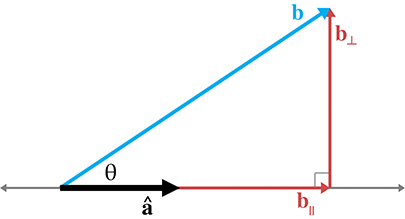
\includegraphics{02_vector_projection}
\caption{Vector projection}
\label{fig:vector-projection}
\end{figure}

\subsubsection{Visibility}

Using the sign of the dot product we can determine where two vectors are in relation to each other.

\begin{figure}[H]
\centering
    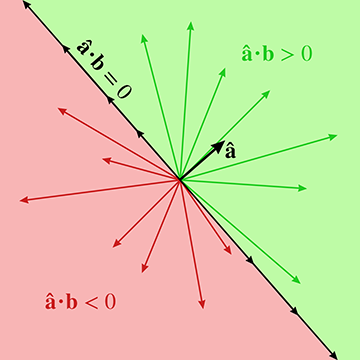
\includegraphics{02_dot_signs}
\caption{Dot product signs}
\label{fig:dot-product-signs}
\end{figure}

\begin{itemize}
	\item A positive dot product means $\textbf{b}$ is in front of $\textbf{a}$.
	\item A negative dot product means $\textbf{b}$ is behind $\textbf{a}$.
	\item A dot product with value 0 means that $\textbf{b}$ is exactly to the left or right of $\textbf{a}$.
\end{itemize}

Some nice calculations and practice with this concept can be found in exercises 20 and 21 of chapter 2. These exercises take distance and field of view into account.

\subsubsection{Cosine angle between two vectors}

The final interpretation is to calculate the angle between two vectors using the dot product. The first thing to remember is that $\cos\theta=\frac{\text{adjecent}}{\text{hypotenuse}}$. With the dot product we calculate how much one vector projects on to the other, thus calculating the adjacent value and creating a right triangle as shown in the image below. Assuming unit vectors as shown in the image we derive $\cos\theta=\frac{\text{adjecent}}{\text{hypotenuse}}=\frac{\hat{\textbf{a}}\cdot\hat{\textbf{b}}}{1}=\hat{\textbf{a}}\cdot\hat{\textbf{b}}$. The general formula that does not assume unit vectors is therefore:

$$\cos\theta=\frac{\hat{\textbf{a}}\cdot\hat{\textbf{b}}}{\|\textbf{a}\|\|\textbf{b}\|}$$

Then to get the actual angle:

$$\theta=\arccos\left(\frac{\hat{\textbf{a}}\cdot\hat{\textbf{b}}}{\|\textbf{a}\|\|\textbf{b}\|}\right)$$

\begin{figure}[H]
\centering
    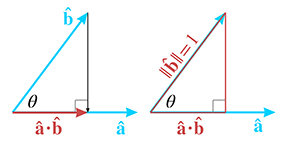
\includegraphics{02_dot_angle}
\caption{Dot product angle}
\label{fig:dot-product-angle}
\end{figure}

Now we can put all this angle calculation into perspective. Take a look at the following table which shows exactly why we were able to use the sign of the dot product to determine if if two vectors are visible with respect to each other.

\begin{table}[H]
\centering
\begin{tabular}{|l|l|l|l|l|}
\hline
$\textbf{a}\cdot\textbf{b}$ & $\theta$ & \textbf{Angle is} & $\textbf{a}$ \textbf{and} $\textbf{b}$ \textbf{are}  \\ \hline
$>0$ & $0^\circ \leq \theta < 90^\circ$ & acute & pointing mostly in the same direction. \\ \hline
$0$ & $\theta=90^\circ$ & right & perpendicular \\ \hline
$<0$ & $90^\circ < \theta \leq 180^\circ$ & obtuse & pointing mostly in the same direction \\ \hline
\end{tabular}
\caption{Dot product angles}
\label{tab:dot-product-angles}
\end{table}

\subsubsection{Magnitude}

A nice thing to realize is that taking the dot product of a vector itself results into the square of its magnitude: $\textbf{v}\cdot\textbf{v}=\|\textbf{v}\|^2$, so $\|\textbf{v}\|=\sqrt{\textbf{v}\cdot\textbf{v}}$.

\subsection{Cross product}

The cross product is slightly more difficult to calculate and does not exist for two dimensional vectors. Unlike the dot product the cross product does not return a scalar, but a vector instead. The general formula is:

$$
\textbf{a}\times\textbf{b}=
\begin{bmatrix}
a_x \\ a_y \\ a_z
\end{bmatrix}\times
\begin{bmatrix}
b_x \\ b_y \\ b_z
\end{bmatrix}=
\begin{bmatrix}
a_yb_z - a_zb_y \\ a_zb_x - a_xb_z \\ a_xb_y - a_yb_x
\end{bmatrix}
$$

\subsubsection{Perpendicular vector}

The geometric interpretation of the cross product is to visualize a third vector perpendicular to the vectors which were used to calculate the cross product. This is for example used to calculate surface normals, but more about that later.

\begin{figure}[H]
\centering
    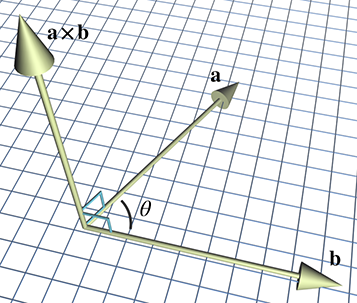
\includegraphics{02_cross_product}
\caption{Cross product}
\label{fig:cross-product}
\end{figure}

\subsubsection{Sine angle between two vectors}

The cross product has a similar usage as the dot product to calculate an angle between two vectors. In this case it is possible to calculate the sine between two vectors as follows: $\sin\theta=\frac{\|\textbf{a}\times\textbf{b}\|}{\|\textbf{a}\|\|\textbf{b}\|}$.
